\section{Introduction}\label{sec:intro}
\sectionstate{open}{the X17 programme at n\_TOF (INTC proposal); \texttt{mpgd26} physics-case figures}
\intent{Why a micro-TPC: the X17 search at n\_TOF needs the $e^+e^-$ opening angle, so each chamber must give a
3D track segment from one drift gap. Why resistive strips (spark protection at the n\_TOF flash). What this paper
covers (design, operation, gas, timing, efficiency, resolution on cosmics and in the SPS beam) and what the
companion paper~\cite{paperII} covers (the reconstruction).}

\tbw{Two or three paragraphs. Cite the ATOMKI anomaly~\cite{Krasznahorkay2016}, the $^3$He(n,$e^+e^-$) calculation~\cite{Viviani2022},
Micromegas~\cite{Giomataris1996} and resistive Micromegas~\cite{Alexopoulos2011}.}

\begin{figure}[t]
  \centering
  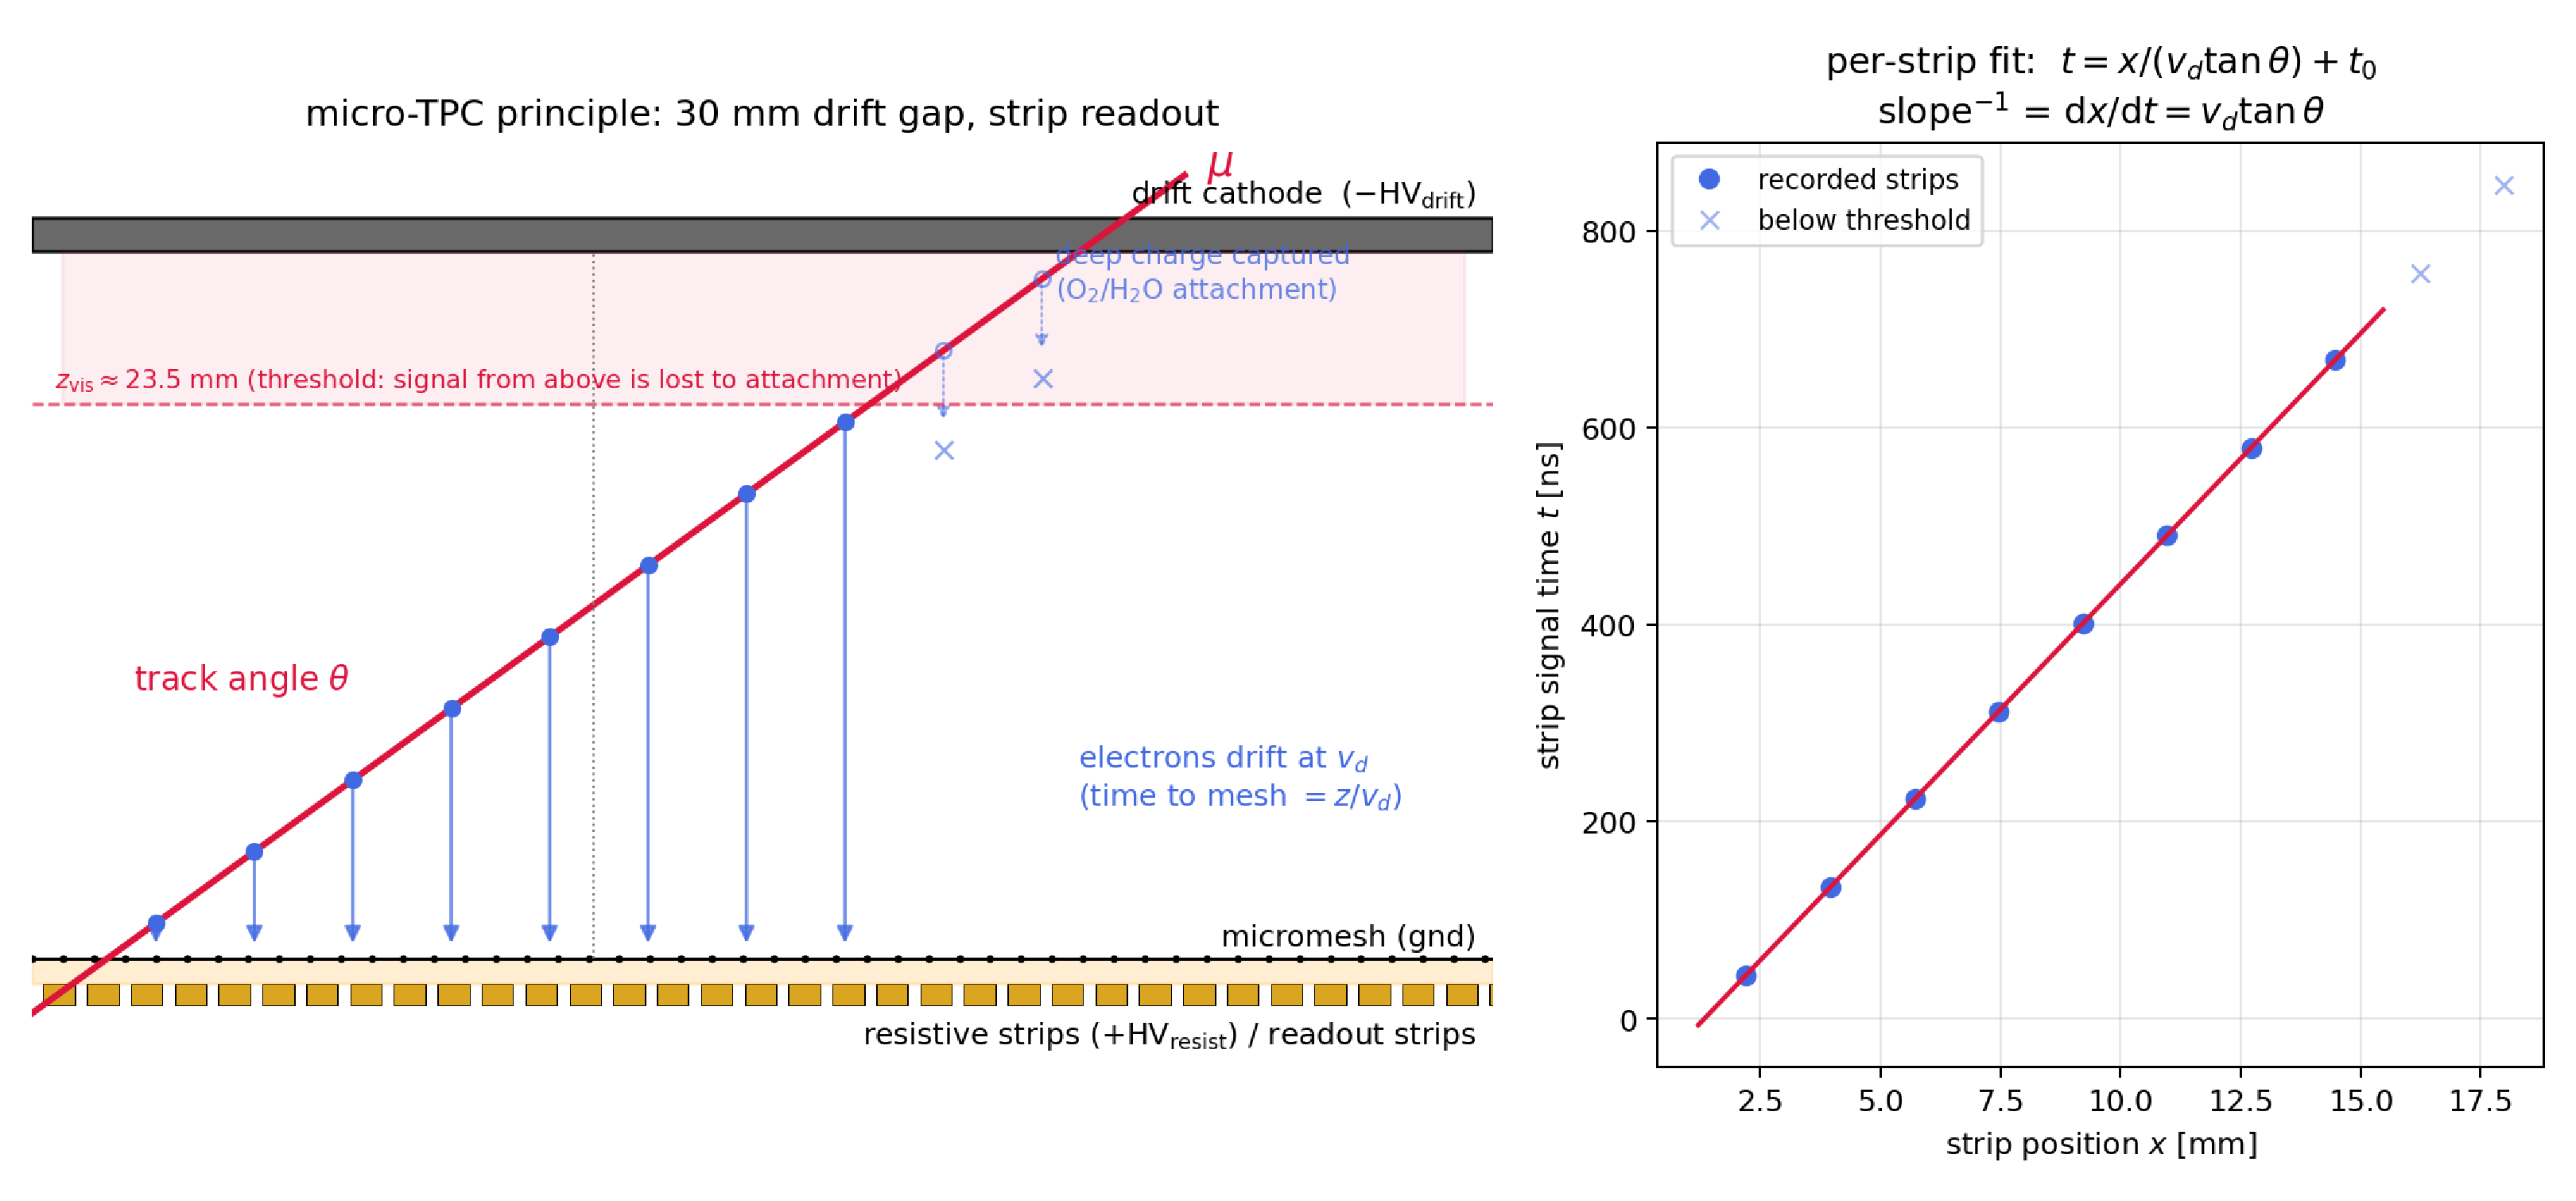
\includegraphics[width=0.85\linewidth]{microtpc_principle}
  \caption{Micro-TPC operation: each strip records the arrival time of its drift electrons, so one 30\,mm gap gives a 3D track segment.}
  \label{fig:microtpc}
\end{figure}
